%%% use twocolumn and 10pt options with the asme2ej format
\documentclass[twocolumn,10pt]{asme2ej}
\usepackage{amssymb}
\usepackage{amsmath}
\usepackage{epsfig} %% for loading postscript figures
\usepackage{graphicx}
\usepackage{algorithm}
\usepackage{algorithmicx, float}
\usepackage{algpseudocode}

\title{De-Mystifying Reduced-Order St. Venant-Kirchhoff Deformable Models}

\author{Gillian P. Reyes
}

\begin{document}

\maketitle

% %%%%%%%%%%%%%%%%%%%%%%%%%%%%%%%%%%%%%%%%%%%%%%%%%%%%%%%%%%%%%%%%%%%%%%
\begin{abstract}
{\it The goal of this paper is to document each step taken in recreating
the results of Real-Time Subspace Integration for St. Venant-Kirchhoff Deformable Models \cite{barbic}, so that
others may use this as a guide to replicate this work.
}
\end{abstract}

% %%%%%%%%%%%%%%%%%%%%%%%%%%%%%%%%%%%%%%%%%%%%%%%%%%%%%%%%%%%%%%%%%%%%%%
\section{Introduction}

The goal of this paper is to document each step taken in recreating Barbič and James's research from their 2005
paper \cite{barbic}. In this research, they utilize past work on real-time deformable objects and model reduction in solid mechanics to speed up computations and allow for large deformations. Finite Element Method is used to discretize partial differential equations of solid continuum mechanics, allowing motion to be described through the Euler-Lagrange equation,

\begin{equation}
M\ddot u + D(u, \dot u) + R(u) = f
\label{eq_motion}
\end{equation}

where $M \in \mathbb{R}^{2n \times 2n }$ is the mass matrix, $D$ is the damping force, $R$ is internal force, and $f$ is external force. $u \in \mathbb{R}^{2n}$ is the displacement vector. This equation is then further reduced by introducing a time-independent matrix, $U \in \mathbb{R}^{2n \times r}$, specifying a basis of some r-dimensional linear subspace. After this reduction, the equation and each of its terms can be solved using:

\begin{equation}
\tilde{M}\ddot q + \tilde{D}(q, \dot q) + \tilde{R}(q) = \tilde{f}
\label{eq_rmotion}
\end{equation}

where $q, \tilde{D}(q, \dot q), \tilde{R}(q), \tilde{f} \in \mathbb{R}^{r}$, $\tilde{M} \in \mathbb{R}^{r \times r}$, and each
can be found through the equations:

\begin{equation}
u = Uq
\label{eq_basisreduction}
\end{equation}
\begin{equation}
\tilde{M} = U^{T}MU
\label{eq_rmass}
\end{equation}
\begin{equation}
\tilde{D}(q, \dot q) = U^{T}D(Uq, U \dot q)
\label{eq_rdamp}
\end{equation}
\begin{equation}
\tilde{R}(q) = U^{T}D(Uq)
\label{eq_rinternal}
\end{equation}
\begin{equation}
\tilde{f} = U^{T}f
\label{eq_rexternal}
\end{equation}
\begin{equation}
\tilde{K} = U^{T}K(Uq)U
\label{eq_rstiffness}
\end{equation}

Using these equations to reduce the problem speeds up the computation of motion to a degree, but everything can be
sped up further if you treat the calculation of $R$ as cubic polynomial and $K$ as a quadratic polynomial. Then,
you can precompute constant coefficients to these equations, such that

\begin{equation}
\tilde{R}(q) = U^{T}R(q) = P^{i}q_{i} + Q^{ij}q_{i}q_{j} + S^{ijk}q_{i}q_{j}q_{k}
\label{eq_rcubicpoly}
\end{equation}

\begin{equation}
\tilde{K}(q) = \frac{\partial \tilde{R}(q)}{\partial q_{l}} = P^{l} + (Q^{li} + Q^{il})q_{i} + (S^{ijl} + S^{ilj} + S^{lij} )q_{i}q_{j}
\label{eq_rquadpoly}
\end{equation}

The reduced Euler-Lagrange equation of motion can then be solved using a Newmark integrator, animating large deformations
of deformable models more efficiently than previously possible.

This paper will start from the very beginning of the process, i.e. creating triangle objects to form a triangle mesh for any
specified model, and walk through every step until an actual animation is created at the end. OpenGL is used for drawing and displaying images, and C++ was used for the rest of the implementation.

% %%%%%%%%%%%%%%%%%%%%%%%%%%%%%%%%%%%%%%%%%%%%%%%%%%%%%%%%%%%%%%%%%%%%%%
\section{An Overview of Tensors}

Before going into the details of how to implement reduced-order St. Venant-Kirchfoff deformable models, it's important to review tensors, as they show up in many places throughout this paper. The following explanation is influenced by Kolda and Bader's paper on Tensor Decomposition and Applications \cite{tensors}, and contains extra findings that emerged through implementation.

A \textbf{tensor} is a multidimensional array. For example, a matrix is a second order tensor, and a vector is a first order tensor. An $N$th order tensor is an array of $N$ dimensions, and thus indexed using $N$ indices.

%%%%%%%%%%%%%%%% begin figure %%%%%%%%%%%%%%%%%%%
%%% 3.34in is the maximum width you can have for a figure
\begin{figure}
\center{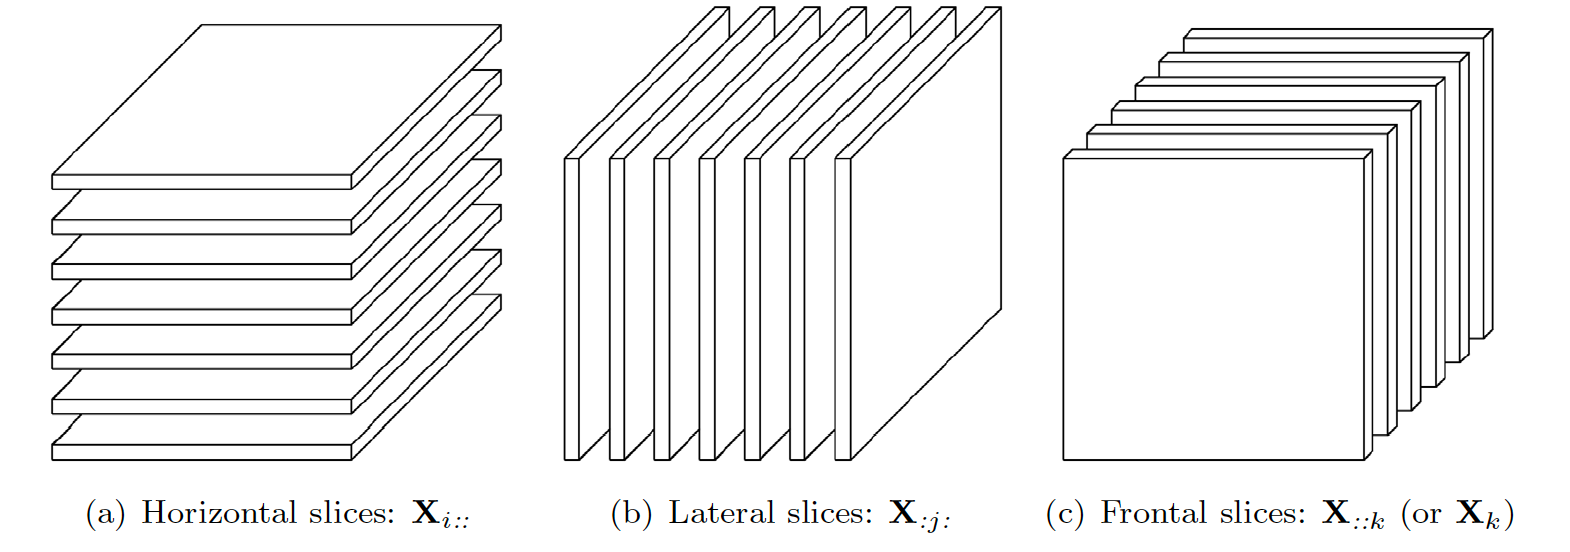
\includegraphics[keepaspectratio,width=4.8in, natwidth = 1570, natheight = 552]{figure/fig1.png}}
\caption{A visual representation of a third order tensor. It can be imagined in three distinct ways, depending on how you index it}
\label{fig_ex1.png}
\end{figure}
%%%%%%%%%%%%%%%% end figure %%%%%%%%%%%%%%%%%%%
%%%%%%%%%%%%%%%% begin figure %%%%%%%%%%%%%%%%%%%
%%% 3.34in is the maximum width you can have for a figure
\begin{figure}
\center{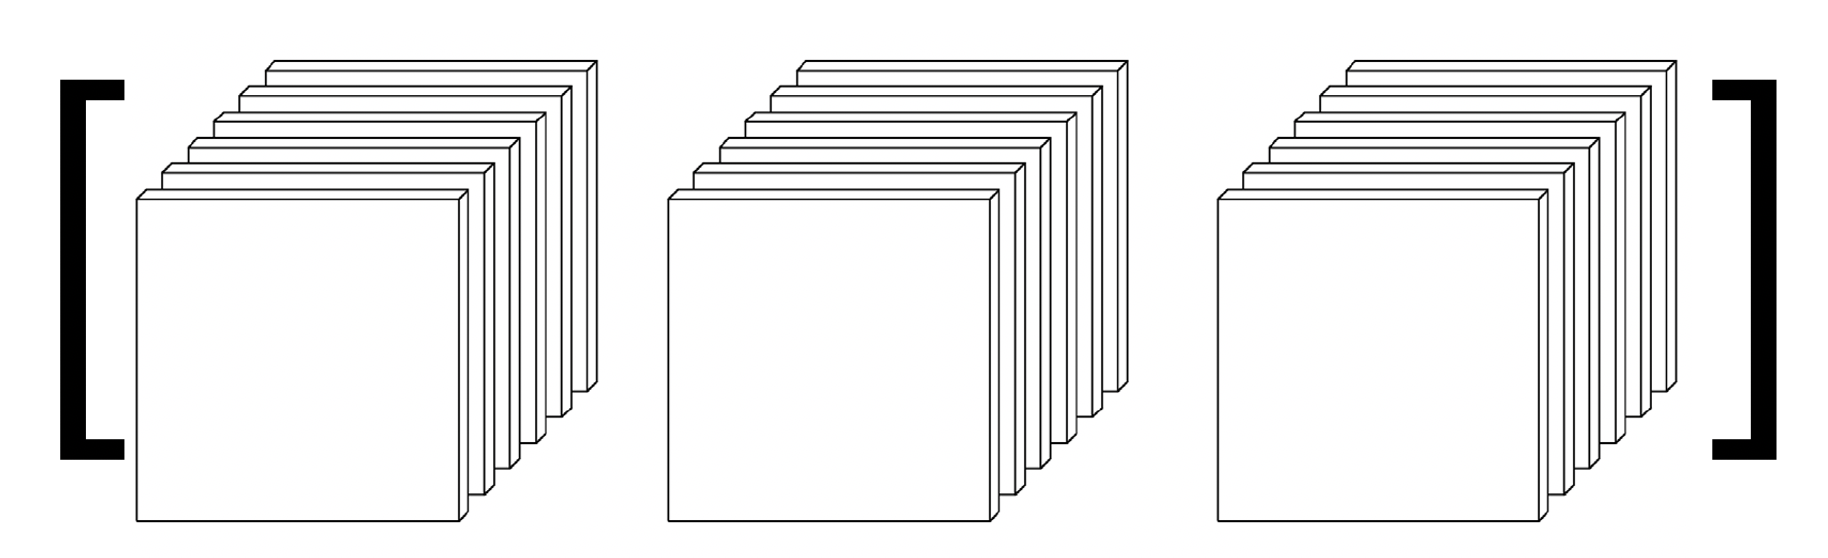
\includegraphics[keepaspectratio,width=4.8in, natwidth = 1828, natheight = 558]{figure/fig2.png}}
\caption{A visual representation of a fourth order tensor. In code, it is treated as a vector of third order tensors.}
\label{fig_ex2.png}
\end{figure}
%%%%%%%%%%%%%%%% end figure %%%%%%%%%%%%%%%%%%%

Figure~\ref{fig_ex1.png} shows a visual representation of a third order tensor; it can be imagined as a vector of matrices, where each square slice represents an individual matrix. Figure~\ref{fig_ex2.png} shows a visual representation of a fourth
order tensor, or a vector of third order tensors. Fourth order tensors are the highest dimension tensor needed for this paper, so no other tensor visuals are included.

There are three different kinds of tensor multiplication that we will use throughout this paper.

\subsection{Scalar Multiplication}

This works exactly as it seems like it would. For $a \in \mathbb{R}$, $X \in \mathbb{R}^{I_1 \times I_2 \times ... \times I_N}$,

\begin{equation}
(aX)_{i_1, i_2, ..., i_n} = a*x_{i_1, i_2, ..., i_n}
\end{equation}

%%%%%%%%%%%%%%%% begin figure %%%%%%%%%%%%%%%%%%%
%%% 3.34in is the maximum width you can have for a figure
\begin{figure}
\center{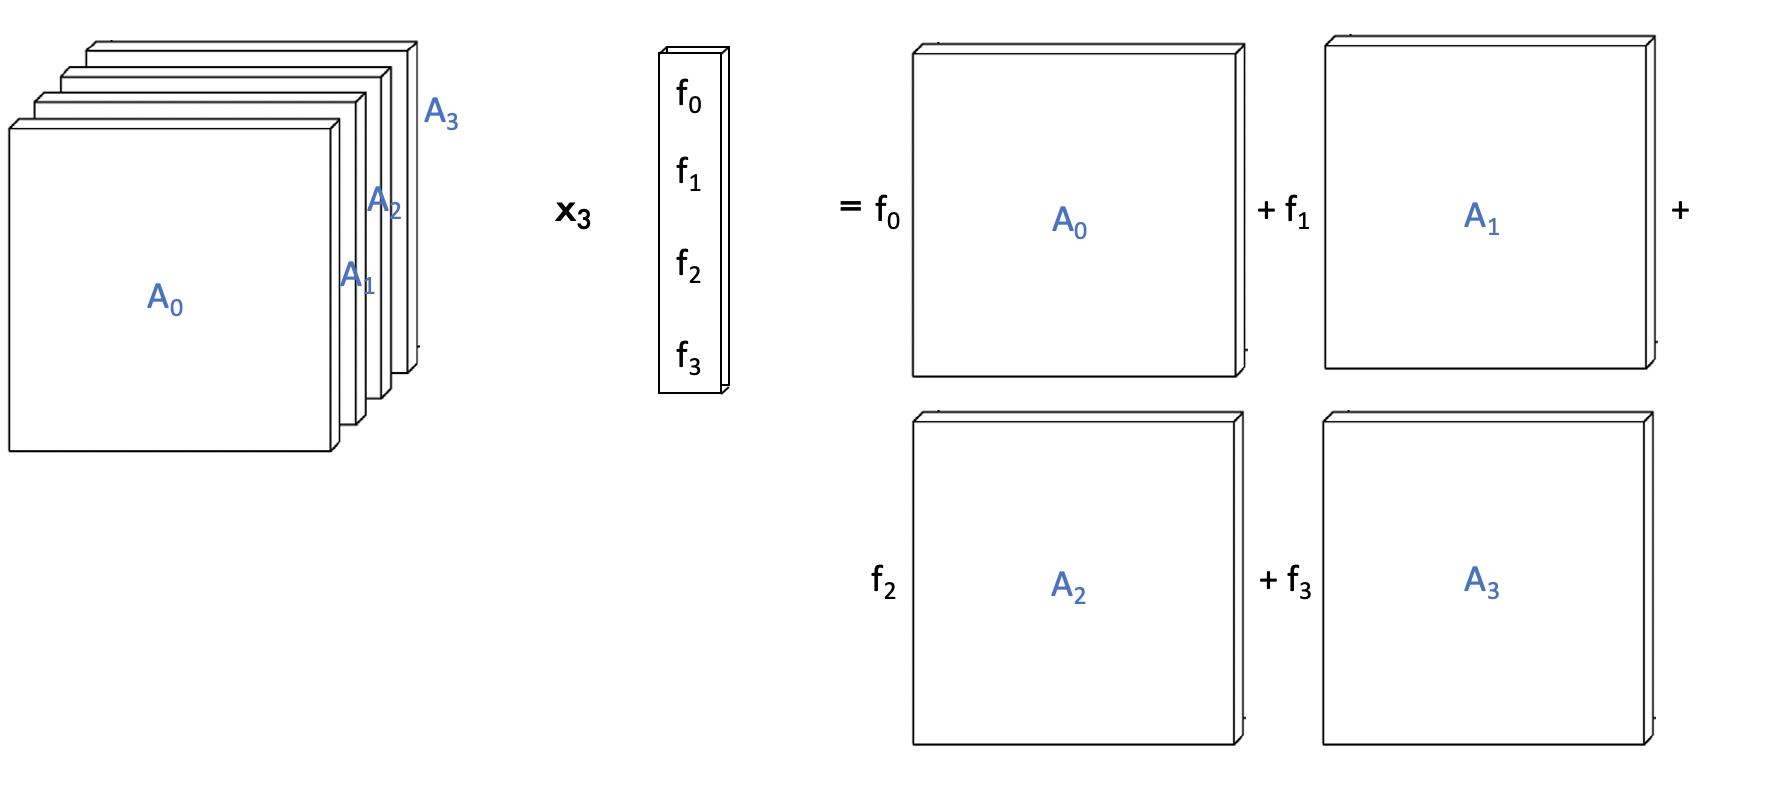
\includegraphics[keepaspectratio,width=4.8in, natwidth = 1774, natheight = 788]{figure/fig3.png}}
\caption{A visual representation of a 3-mode vector product, where $A \in \mathbb{R}^{n \times n \times 4}$ and $f \in \mathbb{R}^{4}$}
\label{fig_ex3.png}
\end{figure}
%%%%%%%%%%%%%%%% end figure %%%%%%%%%%%%%%%%%%%

\subsection{n-Mode Vector Product}

When a tensor is multiplied by a vector, its order reduces by 1. An n-mode vector product of a tensor $X \in \mathbb{R}^{I_1 \times I_2 \times ... \times I_N}$ with a vector $v \in \mathbb{R}^{I_n}$ is denoted by $X \bar{\times}_n v$. Elementwise,

\begin{equation}
(X \bar{\times}_n v )_{i_1, ..., i_{n-1}, i{n+1}, ..., i_N} = \sum_{i_n = 1}{I_n} x_{i_1, i_2, ..., i_N}*v_{i_n}
\end{equation}

So the resulting tensor $(X \bar{\times}_n v ) \in \mathbb{R}^{I_1 \times ... \times I_{n-1} \times I_{n+1} \times ... \times I_N}$. A visual representation of a 3-mode vector product can be seen in Figure~\ref{fig_ex3.png}.
For n-mode vector products, precedence matters, since it change which dimension of the tensor is collapsed. Therefore, if $m < n$,

\begin{equation}
X \bar{\times}_m a \bar{\times}_n b = (X \bar{\times}_m a) \bar{\times}_{n-1} b = (X \bar{\times}_n b) \bar{\times}_m a
\label{eq_vectorMode}
\end{equation}

This is an important rule that will be used later.

\subsection{n-Mode Matrix Product}
When a tensor is multiplied by a matrix, one of its dimensions changes. An n-mode matrix product of a tensor $X \in \mathbb{R}^{I_1 \times I_2 \times ... \times I_N}$ with a matrix $U \in \mathbb{R}^{J \times I_n}$ is denoted by $X \times_n U$. Elementwise, this multiplication results in:

\begin{equation}
(X \times_n U )_{i_1, ..., i_{n-1}, j, i{n+1}, ..., i_N} = \sum_{i_n = 1}{I_n} x_{i_1, i_2, ..., i_N}*u_{j,i_n}
\end{equation}

and the resulting tensor $(X \times_n U ) \in \mathbb{R}^{I_1 \times ... \times I_{n-1} \times J \times I_{n+1} \times ... \times I_N}$.

If $n \neq m$, then

\begin{equation}
X \times_n A \times_m  B = X \times_m B \times_n A
\label{eq_matrixModeCommute}
\end{equation}

If the modes are the same, then

\begin{equation}
X \times_n A \times_n  B = X \times_n (BA)
\label{eq_matrixModeAssociate}
\end{equation}

These two rules will also be used later. Another important rule which will be used later is, for  a tensor $X \in \mathbb{R}^{I_1 \times I_2 \times ... \times I_N}$, a matrix $A \in \mathbb{R}^{I_n, J}$, and a vector $b \in \mathbb{R}^{J}$,

\begin{equation}
X \bar{\times}_n (Ab) = X \times_n A^T \bar{\times}_n b
\label{eq_productDecompose}
\end{equation}

% %%%%%%%%%%%%%%%%%%%%%%%%%%%%%%%%%%%%%%%%%%%%%%%%%%%%%%%%%%%%%%%%%%%%%%
\section{Creating the Triangles}

When modelling solids using a discrete method, the model is represented by a mesh of polygons. In this paper, triangles were
used, so all results of this paper are based on triangle calculations.

In the code for this paper, a triangle object was created for cleaner implementation. Important variables to keep track of are:
\begin{enumerate}
  \item a vector of rest vertices. This should stay constant throughout the simulation.
  \item a vector of actual positions, which update as the whole mesh moves.
  \item a material model of some sort, to keep track of lambda and mu values for force calculations.
  \item rest area; this is used in calculating the internal force and stiffness matrix.
  \item precomputed coefficients for the cubic polynomial interpretation of internal force and quadratic polynomial
  for the tangent stiffness matrix. This will be discussed in a later section.
\end{enumerate}

In addition to storing variables, there are a few useful functions that can go into this object as well:
\begin{enumerate}
  \item getter/setter functions for all private variables.
  \item a function that computes $\frac{\partial F}{\partial u}$.
  \item a function that computes the deformation gradient, $F$.
  \item a function to compute the internal force for the triangle given the deformation gradient.
  \item a function to compute the force jacobian for the triangle given the deformation gradient.
\end{enumerate}

The last three functions are not necessary for the cubic polynomial approach, but are useful for debugging purposes.
All terms used in this section will be explained in the following subsections, which will go into more details of
implementation.

% %%%%%%%%%%%%%%%%%%%%%%%%%%%%%%%%%%%%%%%%%%%%%%%%%%%%%%%%%%%%%%%%%%%%%%
\subsection{Computing the Deformation Gradient}

When a solid is deformed, the \textbf{Deformation Gradient}, $F \in \mathbb{R}^{2 \times 2}$, is the linear mapping from a rest vertex to its deformed position (without translation). This mapping can be used in the calculation of strain energy, so it's an important value to calculate if the cubic polynomial approach is not being used.

The deformation gradient can be found using the equation:

\begin{equation}
F = D_sD_{m}^{-1} = \begin{bmatrix} (x_2 - x_0) & (x_4 - x_0) \\ (x_3 - x_1) & (x_5 - x_1) \end{bmatrix} D_{m}^{-1} = \begin{bmatrix} f_0 & f_2 \\ f_1 & f_3 \end{bmatrix}
\label{eq_F}
\end{equation}

Where $D_s$ is the spatial matrix made of the deformed vertices, $D_m$ is the material matrix made of the rest vertices, and the three vertices of the triangle are $(x_0, x_1), (x_2, x_3), (x_4, x_5)$. Since the rest vertices stay constant throughout the simulation, $D_{m}^{-1}$ is constant.

% %%%%%%%%%%%%%%%%%%%%%%%%%%%%%%%%%%%%%%%%%%%%%%%%%%%%%%%%%%%%%%%%%%%%%%
\subsection{Implementing StVK}

This section is not necessary for the cubic polynomial approach, but it's useful as a debugging tool. In the code
for this paper, the implementation of StVK is tied to the material of the triangle, and is called by the functions
that calculate internal force and the force jacobian for an individual triangle.

A St. Venant-Kirchhoff deformable model is defined by the StVK strain energy, where

\begin{equation}
\psi = \mu ||F^TF - I||^2 + \frac{\lambda}{2}tr(F^TF - I)^2
\label{eq_stvk}
\end{equation}

, and $\lambda$ and $\mu$ are Lamé coefficients.

In computing the internal force of a single triangle, the Piola-Kirchhoff stress tensor, i.e. the derivative of the strain energy by the deformation gradient, is used. The Piola-Kirchhoff stress tensor is

\begin{equation}
\frac{\partial \psi}{\partial F} = 4\mu FF^TF - 4\mu F + 2\lambda Ftr(F^TF) -4\lambda F
\label{eq_pk1}
\end{equation}

In computing the force jacobian of a single triangle, the energy hessian is used. The energy hessian is:

\begin{equation}
  \begin{split}
\frac{\partial^2 \psi}{\partial F^2} = 4\mu [\frac{\partial F}{\partial F_i}F^TF + F\frac{\partial F}{\partial F_i}^TF + FF^T\frac{\partial F}{\partial F_i}] \\ + 2\lambda \frac{\partial F}{\partial F_i}tr(F^TF) - 4[\mu + \lambda]I
  \end{split}
\label{eq_dpdf}
\end{equation}

% %%%%%%%%%%%%%%%%%%%%%%%%%%%%%%%%%%%%%%%%%%%%%%%%%%%%%%%%%%%%%%%%%%%%%%
\subsection{Computing dF/dx}

Before we can calculate internal force and the force jacobian, we need to find the derivative of F in terms of x. Remember that $F \in \mathbb{R}^{2 \times 2}$ and $x \in \mathbb{R}^6$. This means that

\begin{equation}
  \begin{split}
    \frac{\partial F}{\partial x} = \begin{bmatrix} \frac{\partial F}{\partial x_0} & \frac{\partial F}{\partial x_1}
    & \frac{\partial F}{\partial x_2} & \frac{\partial F}{\partial x_3} & \frac{\partial F}{\partial x_4}
    & \frac{\partial F}{\partial x_5} \end{bmatrix} \\
    = \begin{bmatrix} \begin{bmatrix} -1 & -1 \\ 0 & 0 \end{bmatrix} & \begin{bmatrix} 0 & 0 \\ -1 & -1 \end{bmatrix}
  & \begin{bmatrix} 1 & 0 \\ 0 & 0 \end{bmatrix} & \begin{bmatrix} 0 & 0 \\ 1 & 0 \end{bmatrix}
  & \begin{bmatrix} 0 & 1 \\ 0 & 0 \end{bmatrix} & \begin{bmatrix} 0 & 0 \\ 0 & 1 \end{bmatrix}\end{bmatrix}
  \end{split}
\label{eq_dFdx}
\end{equation}

This was derived using equation~\ref{eq_F} for $F$. Notice that this is a vector of matrices, i.e. a third order tensor. While we can use this as a third order tensor, it's easier to vectorize it and treat it as a matrix.

% %%%%%%%%%%%%%%%%%%%%%%%%%%%%%%%%%%%%%%%%%%%%%%%%%%%%%%%%%%%%%%%%%%%%%%
\subsubsection{Flattening Matrices and Tensors}

Flattening a tensor reduces it into a matrix, and flattening a matrix reduces it into a vector (also called vectorizing). To vectorize a matrix, we append the next column onto the bottom of the previous. So, as an example, if

\bigskip
\begin{center}
$A = \begin{bmatrix} 1 & 3 \\ 2 & 4 \end{bmatrix}$
\end{center}

then

\begin{center}
$vec(A) = \begin{bmatrix} 1 \\ 2 \\ 3 \\ 4 \end{bmatrix}$
\end{center}

To flatten a tensor, we do this process on each level - so if we have a fourth order tensor, or a matrix of matrices, we first flatten the outer matrix into a vector of matrices, then vectorize the matrices inside. This step, which is the same for both third and fourth order tensors, can be done as shown below:

\bigskip
\begin{center}
$A = \begin{bmatrix} \begin{bmatrix} 1 & 3 \\ 2 & 4 \end{bmatrix} & \begin{bmatrix} 5 & 7 \\ 6 & 8 \end{bmatrix} \end{bmatrix}$
\end{center}

then

\begin{center}
$vec(A) = \begin{bmatrix} vec(\begin{bmatrix} 1 & 3 \\ 2 & 4 \end{bmatrix}) & vec(\begin{bmatrix} 5 & 7 \\ 6 & 8 \end{bmatrix}) \end{bmatrix} = \begin{bmatrix} 1 & 5 \\ 2 & 6 \\ 3 & 7 \\ 4 & 8 \end{bmatrix}$
\end{center}

% %%%%%%%%%%%%%%%%%%%%%%%%%%%%%%%%%%%%%%%%%%%%%%%%%%%%%%%%%%%%%%%%%%%%%%
\subsection{Computing Internal Force and the Force Jacobian (The Non-Polynomial Way)}

This section is unnecessary for the cubic polynomial approach, but as with all the other sections, it's useful for debugging purposes. The internal force inside of the triangle can be computed using the equation

\begin{equation}
f = \frac{\partial \psi}{\partial u} = vec(\frac{\partial F}{\partial x})^T*vec(\frac{\partial \psi}{\partial F})
\label{eq_triforce}
\end{equation}

where the terms are defined by equations \ref{eq_dFdx} and \ref{eq_pk1}, respectively. The force jacobian for each triangle can be computed using the equation

\begin{equation}
\frac{\partial^2 \psi}{\partial u^2} = vec(\frac{\partial F}{\partial x})^T*\frac{\partial^2 \psi}{\partial F^2}*vec(\frac{\partial F}{\partial x})
\label{eq_trijacob}
\end{equation}

where the terms are defined by equations \ref{eq_dFdx} and \ref{eq_dpdf}. Notice how $x$, or current vertex placement, and $u$, vertex \textit{displacement}, are used interchangably here. In general, this is possible because the interal force at rest position $\bar{x}$ is $0$, and $x = \bar{x} + u$. However, it is important to note, because these will \textbf{not} be interchangable in the cubic polynomial approach.

% %%%%%%%%%%%%%%%%%%%%%%%%%%%%%%%%%%%%%%%%%%%%%%%%%%%%%%%%%%%%%%%%%%%%%%

\section{Creating the Triangle Mesh}

Now that a triangle object has been established, a triangle mesh can be built. In the code for this paper, the triangle mesh is a separate object from the individual triangles, and it stores all of the triangles in a vector. When constructing the triangle mesh, it may be useful to store a map of each vertex to its global position, so that future calculations are easier. In this implementation, the following were stored as private variables:

\begin{enumerate}
  \item a vector of triangles, i.e. the triangle mesh.
  \item a vertex to global index mapping.
  \item a vector of vertex placements.
  \item a vector of vertex rest positions.
  \item a vector of vertex displacements.
  \item a vector of vertex indices representing which vertices are \textbf{constrained}.
  \item a vector of vertex indices representing which vertices are \textbf{unconstrained}.
  \item a vector for inteneral force.
  \item a vector for external force.
  \item a mass matrix.
  \item a vector for velocity and a vector for acceleration.
  \item the basis reduction matrix.
  \item a vector for the reduced basis vector.
\end{enumerate}

% %%%%%%%%%%%%%%%%%%%%%%%%%%%%%%%%%%%%%%%%%%%%%%%%%%%%%%%%%%%%%%%%%%%%%%
\section{Implementing the Euler-Lagrange Equation of Motion}

After setting up the triangle mesh and applying some kind of external force,the system is animated by solving the Euler-Lagrange Equation of Motion. By solving equation~\ref{eq_motion}, the displacements for the next time step can be found and added to the vertex placements. In order to do this, each term of the equation must be calculated.

% %%%%%%%%%%%%%%%%%%%%%%%%%%%%%%%%%%%%%%%%%%%%%%%%%%%%%%%%%%%%%%%%%%%%%%
\subsection{Implementing Internal Force}

While this step isn't necessary for the cubic polynomial approach, the methods are similar. In the previous section, the individual internal force for each triangle was calculated using equation~\ref{eq_triforce}. To calculate the global internal force, $R(u) \in \mathbb{R}^{2n}$, all of the individual internal forces are added up. This can be done by looping through every triangle, then looping through every vertex of the triangle. For each vertex, find where it belongs in the global context, and, if it is not constrained, add the force to the global vector. Here's an example through pseudocode below:

\begin{algorithmic}[1]
    \Function{globalInternalForce}{$null$}
        \State $global\_vector.setZero()$
        \For{triangle in triangles}
         \State $force \gets triangle.force()$
          \For{vertex in triangle vertices}
              \If {vertex is unconstrained}
                  \State $i \gets global\_index(vertex)$
                  \State add to global vector
              \EndIf
            \EndFor
        \EndFor
    \EndFunction
\end{algorithmic}

% %%%%%%%%%%%%%%%%%%%%%%%%%%%%%%%%%%%%%%%%%%%%%%%%%%%%%%%%%%%%%%%%%%%%%%
\subsection{Implementing the Tangent Stiffness Matrix}

The process here is similar to the process of calculating the global internal force. In the previous section, the individual force jacobian for each triangle was calculated using equation~\ref{eq_trijacob}. To calculate the global stiffness matrix, $K(u) \in \mathbb{R}^{2n \times 2n}$, all of the individual force jacobians are added up. This can be done by looping through every triangle, then looping through every vertex of the triangle twice. For each vertex, find where it belongs in the global context, and, if it is not constrained, add the force to the global stiffness matrix. Here's an example through pseudocode below:

\begin{algorithmic}[1]
    \Function{globalStiffnessMatrix}{$null$}
        \State $global\_stiffness.setZero()$
        \For{triangle in triangles}
         \State $jacobian \gets triangle.jacobian()$
          \For{$vertex$ in triangle vertices}
              \If {$vertex$ is unconstrained}
                  \State $i \gets global\_index(vertex)$
                  \For{$vertex_2$ in triangle vertices}
                      \If {$vertex_2$ is unconstrained}
                          \State $j \gets global\_index(vertex_2)$
                          \State add to global stiffness matrix
                      \EndIf
                    \EndFor
              \EndIf
            \EndFor
        \EndFor
    \EndFunction
\end{algorithmic}

% %%%%%%%%%%%%%%%%%%%%%%%%%%%%%%%%%%%%%%%%%%%%%%%%%%%%%%%%%%%%%%%%%%%%%%
\subsection{Implementing the Mass Matrix}

The mass matrix does not change over time, so this can be initialized outside of the motion function. How mass is implemented is up to the creator.

% %%%%%%%%%%%%%%%%%%%%%%%%%%%%%%%%%%%%%%%%%%%%%%%%%%%%%%%%%%%%%%%%%%%%%%
\subsection{Implementing the Damping Matrix}

The damping matrix is calculated using the equation

\begin{equation}
D(u) = (\alpha M + \beta K(u))
\label{eq_damp}
\end{equation}

After computing the global stiffness matrix, this should be straightforward. The alpha and beta values are constant values that are up to the creator, depending on how strong the desired force is.

% %%%%%%%%%%%%%%%%%%%%%%%%%%%%%%%%%%%%%%%%%%%%%%%%%%%%%%%%%%%%%%%%%%%%%%
\subsection{Implementing the Newmark Integrator}

After calculating all of the individual terms in the Euler-Lagrange equation of motion, the equation can be solved for a given timestep using an implicit Newmark integrator. Implicit Newmark integrators are second-order accurate, and they only require one step, instead of having to solve the equation in a few iterations. While the pseudocode below is written for unreduced displacements, this iteration stays exactly the same when $u$ is replaced with $q$.

\begin{algorithmic}[1]
    \Function{NewmarkIntegrator}{$null$}
      \State $u_{i + 1} \gets u_i$
      \State Evaluate internal forces $R(u_i)$
      \State Evaluate the stiffness matrix $K(u_i)$
      \State Calculate the damping matrix, $D(u_i) = \alpha M + \beta K$
      \State Calculate the system matrix, $A = \alpha_1M + \alpha_4D(u_i) - K$
      \State residual $\gets (\alpha_3M - \alpha_6D)\ddot u_{i} + (\alpha_2M - \alpha_5D)\dot u_{i} + R(u_i) + f_{i+1}$
      \State $ \Delta u \gets A^{-1} *$ residual
      \State $ u_{i + 1} \gets u_{i + 1} + \Delta u$
      \State $ \dot u_{i + 1} \gets \alpha_4(u_{i+1} - u_i) + \alpha_5 \dot u_i + \alpha_6 \ddot u_i$
      \State $ \ddot u_{i + 1} \gets \alpha_1(u_{i+1} - u_i) - \alpha_2 \dot u_i - \alpha_3 \ddot u_i$
    \EndFunction
\end{algorithmic}

The alpha constants in this integrator are determined by the equations

\begin{center}
$\alpha_1 = \frac{1}{\tilde{\beta}(\Delta t)^2}, \alpha_2 = \frac{1}{\tilde{\beta}\Delta t},
\alpha_3 = \frac{1 - 2\tilde{\beta}}{2\tilde{\beta}}, \alpha_4 = \frac{\tilde{\gamma}}{\tilde{\beta}\Delta t},$

$\alpha_5 = 1 - \frac{\tilde{\gamma}}{\tilde{\beta}}, \alpha_6 = (1 - \frac{\tilde{\gamma}}{2\tilde{\beta}})\Delta t$
\end{center}

Where $0 \leq \tilde{\beta} \leq 0.5$ and $0 \leq \tilde{\gamma} \leq 1$. I chose $\tilde{\beta} = 0.25$ and $\tilde{\gamma} = 0.5$ for this implementation, but Barbič and James chose $\tilde{\beta} = 0$ and $\tilde{\gamma} = 0.5$.

% %%%%%%%%%%%%%%%%%%%%%%%%%%%%%%%%%%%%%%%%%%%%%%%%%%%%%%%%%%%%%%%%%%%%%%
\section{Generating Precomputed Coefficients}

At this point in the paper, a fully function simulator of St. Venant-Kirchhoff deformable models can be created; however, they are still unreduced and lack any precomputation. If precomputation does not interest you, feel free to skip to the section titled \textbf{Generating a Deformation Basis} - after creating a deformation basis, reducing everything is as simple as following equations \ref{eq_basisreduction} - \ref{eq_rstiffness}.

For simplicity, I derived the precomputed constant coefficients before reducing the equation. In order to have the ability to precompute constant coefficients, all variables must be extractable. In the case of unreduced St. Venant Kirchhoff models, this means that we should be able to separate vertex positions, $x$, out of the internal force and stiffness matrix calculation. Again, for simplicity, I began by separating $x$ from the internal force equation \ref{eq_triforce} and force jacobian equation \ref{eq_trijacob} for an individual triangle, then created global constants similar to how the global internal force and global stiffness matrix were built in sections 5.1 and 5.2.

% %%%%%%%%%%%%%%%%%%%%%%%%%%%%%%%%%%%%%%%%%%%%%%%%%%%%%%%%%%%%%%%%%%%%%%
\subsection{Coefficients for the Tangent Stiffness Matrix}

Looking at equation~\ref{eq_dpdf}, there is clearly one quadratic term, and one constant matrix, $-4[\mu + \lambda]I$. From this, we can already derive the constant coefficient term:

\begin{equation}
  Q = - vec(\frac{\partial F}{\partial x})^T 4[\mu + \lambda]I vec(\frac{\partial F}{\partial x})
  \label{eq_unreducedConst}
\end{equation}

The quadratic term is trickier. Looking at the $\mu$ term of $\frac{\partial^2 \psi}{\partial F^2}$ alone, $[\frac{\partial F}{\partial F_i}F^TF + F\frac{\partial F}{\partial F_i}^TF + FF^T\frac{\partial F}{\partial F_i}]$ decomposes into

\begin{center}
$\frac{\partial F}{\partial F_i}F^TF = \begin{bmatrix} f_{0}^2 + f_{1}^2 & 0 & f_0f_2 + f_1f_3 & 0 \\
0 & f_{0}^2 + f_{1}^2 & 0 & f_0f_2 + f_1f_3 \\
f_0f_2 + f_1f_3 & 0 & f_{2}^2 + f_{3}^2 & 0 \\
0 & f_0f_2 + f_1f_3 & 0 & f_{2}^2 + f_{3}^2 \end{bmatrix}$

\bigskip
$F\frac{\partial F}{\partial F_i}^TF = \begin{bmatrix} f_{0}^2 & f_0f_1 & f_0f_2 & f_1f_2  \\
f_0f_1 & f_{1}^2 & f_0f_3 & f_1f_3 \\
f_0f_2 & f_0f_3 & f_{2}^2 & f_2f_3 \\
f_1f_2 & f_1f_3 & f_2f_3 & f_{3}^2 \end{bmatrix}$

\bigskip
$FF^T\frac{\partial F}{\partial F_i} = \begin{bmatrix} f_{0}^2 + f_{2}^2 & f_0f_1 + f_2f_3 & 0 & 0  \\
f_0f_1 + f_2f_3 & f_{1}^2 + f_{3}^2 & 0 & 0 \\
0 & 0 & f_{0}^2 + f_{2}^2 & f_0f_1 + f_2f_3 \\
0 & 0 & f_0f_1 + f_2f_3 & f_{1}^2 + f_{3}^2 \end{bmatrix}$
\end{center}

In order to separate out all of the $x$'s, we can first separate all of the $f$ terms. It turns out that this can be done using tensors. By working backwards from the matrices above, a fourth order tensors, $C_{\mu}$, can be derived, such that

\begin{equation}
    C_{\mu} = \begin{bmatrix}
    \begin{bmatrix} 3 & 0 & 0 & 0 \\ 0 & 1 & 0 & 0 \\ 0 & 0 & 1 & 0 \\ 0 & 0 & 0 & 0 \end{bmatrix} &
    \begin{bmatrix} 0 & 2 & 0 & 0 \\ 0 & 0 & 0 & 0 \\ 0 & 0 & 0 & 1 \\ 0 & 0 & 0 & 0 \end{bmatrix} &
    \begin{bmatrix} 0 & 0 & 2 & 0 \\ 0 & 0 & 0 & 1 \\ 0 & 0 & 0 & 0 \\ 0 & 0 & 0 & 0 \end{bmatrix} &
    \begin{bmatrix}0 & 0 & 0 & 0 \\ 0 & 0 & 0 & 0 \\ 0 & 1 & 0 & 0 \\ 0 & 0 & 0 & 0 \end{bmatrix} \\
      \begin{bmatrix} 0 & 0 & 0 & 0 \\ 2 & 0 & 0 & 0 \\ 0 & 0 & 0 & 0 \\ 0 & 0 & 1 & 0 \end{bmatrix} &
      \begin{bmatrix} 1 & 0 & 0 & 0 \\ 0 & 3 & 0 & 0 \\ 0 & 0 & 0 & 0 \\ 0 & 0 & 0 & 1 \end{bmatrix} &
      \begin{bmatrix} 0 & 0 & 0 & 0 \\ 0 & 0 & 0 & 0 \\ 0 & 0 & 0 & 0 \\ 1 & 0 & 0 & 0 \end{bmatrix} &
      \begin{bmatrix}0 & 0 & 1 & 0 \\ 0 & 0 & 0 & 2 \\ 0 & 0 & 0 & 0 \\ 0 & 0 & 0 & 0 \end{bmatrix} \\
        \begin{bmatrix} 0 & 0 & 0 & 0 \\ 0 & 0 & 0 & 0 \\ 2 & 0 & 0 & 0 \\ 0 & 1 & 0 & 0 \end{bmatrix} &
        \begin{bmatrix} 0 & 0 & 0 & 1 \\ 0 & 0 & 0 & 0 \\ 0 & 0 & 0 & 0 \\ 0 & 0 & 0 & 0 \end{bmatrix} &
        \begin{bmatrix} 1 & 0 & 0 & 0 \\ 0 & 0 & 0 & 0 \\ 0 & 0 & 3 & 0 \\ 0 & 0 & 0 & 1 \end{bmatrix} &
        \begin{bmatrix}0 & 1 & 0 & 0 \\ 0 & 0 & 0 & 0 \\ 0 & 0 & 0 & 2 \\ 0 & 0 & 0 & 0 \end{bmatrix} \\
          \begin{bmatrix} 0 & 0 & 0 & 0 \\ 0 & 0 & 1 & 0 \\ 0 & 0 & 0 & 0 \\ 0 & 0 & 0 & 0 \end{bmatrix} &
          \begin{bmatrix} 0 & 0 & 0 & 0 \\ 0 & 0 & 0 & 0 \\ 1 & 0 & 0 & 0 \\ 0 & 2 & 0 & 0 \end{bmatrix} &
          \begin{bmatrix} 0 & 0 & 0 & 0 \\ 1 & 0 & 0 & 0 \\ 0 & 0 & 0 & 0 \\ 0 & 0 & 2 & 0 \end{bmatrix} &
          \begin{bmatrix}0 & 0 & 0 & 0 \\ 0 & 1 & 0 & 0 \\ 0 & 0 & 1 & 0 \\ 0 & 0 & 0 & 3 \end{bmatrix} \end{bmatrix}
\label{_eq_quadmu}
\end{equation}

And
\begin{equation}
\begin{split}
4\mu[\frac{\partial F}{\partial F_i}F^TF + F\frac{\partial F}{\partial F_i}^TF + FF^T\frac{\partial F}{\partial F_i}] =
\\ 4\mu C_{\mu} \bar{\times}_4 vec(F) \bar{\times}_3 vec(F)
\end{split}
\end{equation}

Similar to the $\mu$ term, the $\lambda$ term, which can be split into the two terms:

\begin{center}
  $2\lambda (\frac{\partial F}{\partial F_i}tr(F^TF)  = 2\lambda(f_{0}^2 + f_{1}^2 + f_{2}^2  + f_{3}^2) \begin{bmatrix}
  1 & 0 & 0 & 0  \\
  0 & 1  & 0 & 0 \\
  0 & 0 & 1  & 0 \\
  0 & 0 & 0 & 1  \end{bmatrix}$

  \bigskip
  $2\lambda (F\frac{\partial tr(F^TF)}{\partial F_i})  = 2\lambda \begin{bmatrix}
  2f_{0}^2 & 2f_0f_1 & 2f_0f_2 & 2f_0f_3  \\
  2f_0f_1 & 2f_{1}^2 & 2f_1f_2 & 2f_1f_3 \\
  2f_0f_2 & 2f_1f_2 & 2f_{2}^2 & 2f_2f_3 \\
  2f_0f_3 & 2f_1f_3 & 2f_2f_3 & 2f_{3}^2  \end{bmatrix}$
\end{center}

has a fourth order tensors that can be derived:

\begin{equation}
    C_{\lambda} = \begin{bmatrix}
    \begin{bmatrix} 3 & 0 & 0 & 0 \\ 0 & 1 & 0 & 0 \\ 0 & 0 & 1 & 0 \\ 0 & 0 & 0 & 1 \end{bmatrix} &
    \begin{bmatrix} 0 & 2 & 0 & 0 \\ 2 & 0 & 0 & 0 \\ 0 & 0 & 0 & 0 \\ 0 & 0 & 0 & 0 \end{bmatrix} &
    \begin{bmatrix} 0 & 0 & 2 & 0 \\ 0 & 0 & 0 & 0 \\ 2 & 0 & 0 & 0 \\ 0 & 0 & 0 & 0 \end{bmatrix} &
    \begin{bmatrix}0 & 0 & 0 & 2 \\ 0 & 0 & 0 & 0 \\ 0 & 0 & 0 & 0 \\ 2 & 0 & 0 & 0 \end{bmatrix} \\
      \begin{bmatrix} 0 & 0 & 0 & 0 \\ 0 & 0 & 0 & 0 \\ 0 & 0 & 0 & 0 \\ 0 & 0 & 0 & 0 \end{bmatrix} &
      \begin{bmatrix} 1 & 0 & 0 & 0 \\ 0 & 3 & 0 & 0 \\ 0 & 0 & 1 & 0 \\ 0 & 0 & 0 & 1 \end{bmatrix} &
      \begin{bmatrix} 0 & 0 & 0 & 0 \\ 0 & 0 & 2 & 0 \\ 0 & 2 & 0 & 0 \\ 0 & 0 & 0 & 0 \end{bmatrix} &
      \begin{bmatrix}0 & 0 & 0 & 0 \\ 0 & 0 & 0 & 2 \\ 0 & 0 & 0 & 0 \\ 0 & 2 & 0 & 0 \end{bmatrix} \\
        \begin{bmatrix} 0 & 0 & 0 & 0 \\ 0 & 0 & 0 & 0 \\ 0 & 0 & 0 & 0 \\ 0 & 0 & 0 & 0 \end{bmatrix} &
        \begin{bmatrix} 0 & 0 & 0 & 0 \\ 0 & 0 & 0 & 0 \\ 0 & 0 & 0 & 0 \\ 0 & 0 & 0 & 0 \end{bmatrix} &
        \begin{bmatrix} 1 & 0 & 0 & 0 \\ 0 & 1 & 0 & 0 \\ 0 & 0 & 3 & 0 \\ 0 & 0 & 0 & 1 \end{bmatrix} &
        \begin{bmatrix}0 & 0 & 0 & 0 \\ 0 & 0 & 0 & 0 \\ 0 & 0 & 0 & 2 \\ 0 & 0 & 2 & 0 \end{bmatrix} \\
          \begin{bmatrix} 0 & 0 & 0 & 0 \\ 0 & 0 & 0 & 0 \\ 0 & 0 & 0 & 0 \\ 0 & 0 & 0 & 0 \end{bmatrix} &
          \begin{bmatrix} 0 & 0 & 0 & 0 \\ 0 & 0 & 0 & 0 \\ 0 & 0 & 0 & 0 \\ 0 & 0 & 0 & 0 \end{bmatrix} &
          \begin{bmatrix} 0 & 0 & 0 & 0 \\ 0 & 0 & 0 & 0 \\ 0 & 0 & 0 & 0 \\ 0 & 0 & 0 & 0 \end{bmatrix} &
          \begin{bmatrix}1 & 0 & 0 & 0 \\ 0 & 1 & 0 & 0 \\ 0 & 0 & 1 & 0 \\ 0 & 0 & 0 & 3 \end{bmatrix} \end{bmatrix}
\label{_eq_quadlambda}
\end{equation}

And
\begin{equation}
2\lambda[\frac{\partial F}{\partial F_i}tr(F^TF) + F\frac{\partial tr(F^TF)}{\partial F_i}] = 2\lambda C_{\lambda} \bar{\times}_4 vec(F) \bar{\times}_3 vec(F)
\end{equation}

So the entire quadratic term can be written as

\begin{equation}
C_f \bar{\times}_4 vec(F) \bar{\times}_3 vec(F) =  (4\mu C_{\mu} + 2\lambda C_{\lambda}) \bar{\times}_4 vec(F) \bar{\times}_3 vec(F)
\end{equation}

This still only separates $F$, not $x$. However, since $F = \frac{\partial F}{\partial x}x$, we can rearrange this equation using our tensor product rules (equations~\ref{eq_vectorMode}-\ref{eq_productDecompose}) so that
\begin{center}
  \begin{multline}
  C_f \bar{\times}_4 vec(F) \bar{\times}_3 vec(F) = C_f \bar{\times}_4 vec( \frac{\partial F}{\partial x}x) \bar{\times}_3 vec( \frac{\partial F}{\partial x}x)
  \\ = C_f \bar{\times}_4 vec( \frac{\partial F}{\partial x}) vec(x) \bar{\times}_3 vec( \frac{\partial F}{\partial x}) vec(x)
  \\ = C_f \times_4 vec( \frac{\partial F}{\partial x})^T \bar{\times}_4 vec(x) \times_3 vec( \frac{\partial F}{\partial x})^T \bar{\times}_3 vec(x)
  \\ = [C_f \times_4 vec( \frac{\partial F}{\partial x})^T \times_3 vec( \frac{\partial F}{\partial x})^T] \bar{\times}_4 vec(x) \bar{\times}_3 vec(x)
\end{multline}
\end{center}

Since $\frac{\partial F}{\partial x}$ is constant (refer back to equation~\ref{eq_dFdx}), this can be pushed into our constant, so that our final quadratic constant can be written as

\begin{equation}
C  = C_f \times_4 vec( \frac{\partial F}{\partial x})^T \times_3 vec( \frac{\partial F}{\partial x})^T
\label{eq_unreducedQuad}
\end{equation}

% %%%%%%%%%%%%%%%%%%%%%%%%%%%%%%%%%%%%%%%%%%%%%%%%%%%%%%%%%%%%%%%%%%%%%%
\subsubsection{Creating the Global Tangent Stiffness Matrix Coefficients}

Now that the constant terms for the force jacobian for each triangle has been computed, we can create global constant terms for the tangent stiffness matrix in a similar way manner as how the global tangent stiffness matrix was computed earlier.

\begin{algorithmic}[1]
    \Function{globalStiffnessConstants}{$null$}
        \State $Q_{global}.setZero()$
        \State $C_{global}.setZero()$
        \For{triangle in triangles}
         \State $Q \gets triangle.getQ()$
         \State $C \gets triangle.getC()$
          \For{$vertex$ in triangle vertices}
              \If {$vertex$ is unconstrained}
                  \State $i \gets global\_index(vertex)$
                  \For{$vertex_2$ in triangle vertices}
                      \If {$vertex_2$ is unconstrained}
                          \State $j \gets global\_index(vertex_2)$
                          \State $Q_{global}(i,j) \gets Q_{global}(i,j) + Q(vertex, vertex_2)$
                          \For{$vertex_3$ in triangle vertices}
                                \State $k \gets global\_index(vertex_3)$
                                \For{$vertex_4$ in triangle vertices}
                                    \State $l \gets global\_index(vertex_4)$
                                    \State $C_{global}(i,j,k,l)  \gets C_{global}(i,j,k,l)+C(vertex, vertex_2, vertex_3, vertex_4)$
                                  \EndFor
                            \EndFor
                      \EndIf
                    \EndFor
              \EndIf
            \EndFor
        \EndFor
    \EndFunction
\end{algorithmic}

Note that the global coefficients match the order of the triangle coefficients; that is, the constant term, $Q_{global}$ is a matrix, while the global coefficient for the quadratic term, $C_{global}$, is a fourth-order tensor. The difference is in their dimensions; while $Q \in \mathbb{R}^{6 \times 6}$, $Q_{global} \in \mathbb{R}^{2n \times 2n}$, and while  $C \in \mathbb{R}^{6 \times 6 \times 6 \times 6}$, $C_{global} \in \mathbb{R}^{2n \times 2n \times 2n \times 2n}$.

Also note that this pseudocode is abbreviated; while it only shows adding $C$ and $Q$ to one position in the global coefficients, you actually have to add it to every possible combination of the current vertices's $x$ and $y$ coordinates. For example, if $vertex$ and $vertex_2$ are unconstrained, then

\begin{center}
$Q_{global}(i,j) += Q(vertex(x), vertex_2(x))$,

$Q_{global}(i + 1,j) += Q(vertex(y), vertex_2(x))$,

$Q_{global}(i ,j + 1) += Q(vertex(x), vertex_2(y))$, and

$Q_{global}(i + 1,j + 1) += Q(vertex(y), vertex_2(y))$.
\end{center}

% %%%%%%%%%%%%%%%%%%%%%%%%%%%%%%%%%%%%%%%%%%%%%%%%%%%%%%%%%%%%%%%%%%%%%%
\subsection{Coefficients for Internal Force}

Looking at equation~\ref{eq_pk1}, there is clearly one cubic term, and one linear term. Since the force jacobian is the derivative of internal force, the linear coefficient for internal force is actually also $Q$. The connection between the cubic term and the quadratic term, however, is not as clean, because the cubic term can be reduced into a fourth order tensor as well.


% %%%%%%%%%%%%%%%%%%%%%%%%%%%%%%%%%%%%%%%%%%%%%%%%%%%%%%%%%%%%%%%%%%%%%%
\subsubsection{Creating the Global Internal Force Coefficients}

An explanation of how to derive the global internal force.

% %%%%%%%%%%%%%%%%%%%%%%%%%%%%%%%%%%%%%%%%%%%%%%%%%%%%%%%%%%%%%%%%%%%%%%
\section{Generating a Deformation Basis}

An explanation of how to generate a deformation basis.

% %%%%%%%%%%%%%%%%%%%%%%%%%%%%%%%%%%%%%%%%%%%%%%%%%%%%%%%%%%%%%%%%%%%%%%
\section{Reducing the Euler-Lagrange Equation of Motion}

An explanation of how to push U through so that we can reduce the order of our calculations.

% %%%%%%%%%%%%%%%%%%%%%%%%%%%%%%%%%%%%%%%%%%%%%%%%%%%%%%%%%%%%%%%%%%%%%%
\subsection{Reducing the Internal Force}

An explanation of how to reduce the calculation of the internal forces, changing the coefficients
of the polynomial.

% %%%%%%%%%%%%%%%%%%%%%%%%%%%%%%%%%%%%%%%%%%%%%%%%%%%%%%%%%%%%%%%%%%%%%%
\subsection{Reducing the Global Tangent Stiffness Matrix}

An explanation of how to reduce the calculation of the stiffness, changing the coefficients
of the polynomial.

% %%%%%%%%%%%%%%%%%%%%%%%%%%%%%%%%%%%%%%%%%%%%%%%%%%%%%%%%%%%%%%%%%%%%%%
\subsection{Reducing All Other Forces}

An explanation of how to reduce all other forces.

% %%%%%%%%%%%%%%%%%%%%%%%%%%%%%%%%%%%%%%%%%%%%%%%%%%%%%%%%%%%%%%%%%%%%%%
\section{Running the program}

A brief explanation of how to run the program

% %%%%%%%%%%%%%%%%%%%%%%%%%%%%%%%%%%%%%%%%%%%%%%%%%%%%%%%%%%%%%%%%%%%%%%
\section{Conclusions}

End it by explaining how I hope this helps anyone who wants to try implementing this on their own.
Explain how this can probably be optimized further by flattening all tensors.

% %%%%%%%%%%%%%%%%%%%%%%%%%%%%%%%%%%%%%%%%%%%%%%%%%%%%%%%%%%%%%%%%%%%%%%
\begin{acknowledgment}

Thanks to Barbič for writing the paper and my advisor Theodore Kim.

\end{acknowledgment}

%%%%%%%%%%%%%%%%%%%%%%%%%%%%%%%%%%%%%%%%%%%%%%%%%%%%%%%%%%%%%%%%%%%%%%

% Here's where you specify the bibliography style file.
% The full file name for the bibliography style file
% used for an ASME paper is asmems4.bst.
\bibliographystyle{asmems4}

% Here's where you specify the bibliography database file.
% The full file name of the bibliography database for this
% article is asme2e.bib. The name for your database is up
% to you.
\bibliography{writeup}

%%%%%%%%%%%%%%%%%%%%%%%%%%%%%%%%%%%%%%%%%%%%%%%%%%%%%%%%%%%%%%%%%%%%%%
% \appendix       %%% starting appendix
% \section*{Appendix A: Head of First Appendix}
% \begin{center}
%   $2\lambda (\frac{\partial F}{\partial F_i}tr(F^TF)  = 2\lambda(f_{0}^2 + f_{1}^2 + f_{2}^2  + f_{3}^2) \begin{bmatrix}
%   1 & 0 & 0 & 0  \\
%   0 & 1  & 0 & 0 \\
%   0 & 0 & 1  & 0 \\
%   0 & 0 & 0 & 1  \end{bmatrix}$
%
%   \bigskip
%   $2\lambda (F\frac{\partial tr(F^TF)}{\partial F_i})  = 2\lambda \begin{bmatrix}
%   2f_{0}^2 & 2f_0f_1 & 2f_0f_2 & 2f_0f_3  \\
%   2f_0f_1 & 2f_{1}^2 & 2f_1f_2 & 2f_1f_3 \\
%   2f_0f_2 & 2f_1f_2 & 2f_{2}^2 & 2f_2f_3 \\
%   2f_0f_3 & 2f_1f_3 & 2f_2f_3 & 2f_{3}^2  \end{bmatrix}$
% \end{center}

\end{document}
